\documentclass{article}
\usepackage[utf8]{inputenc}
\usepackage[spanish]{babel}

% Formato de página
\usepackage[letterpaper, margin = 1.5cm]{geometry}

% Más opciones para enumerar
\usepackage{enumitem}
\usepackage{amsmath}

% Manejo de imágenes
\usepackage{graphicx}
\usepackage{wrapfig}
\graphicspath{{img/}}
\usepackage{float}

\begin{document}
    \title{
        Fundamentos de bases de datos \\
        Tarea 4 \\
        Álgebra Relacional
    }
    \author{
        Díaz Gómez Silvia \\
        Eugenio Aceves Narciso Isaac \\
        Quiroz Castañeda Edgar
    }
    \date {
        3 de abril del 2019    
    }
    \maketitle

    \begin{enumerate}
        \item {
            Para el problema de la base de datos del \textbf{Museo} que se
            transformó a \textbf{Modelos Relacional} en la tarea anterior,
            verifica que con ésta puedas satisfacer las siguientes consultas.
            \begin{figure}[H]
                \centering
                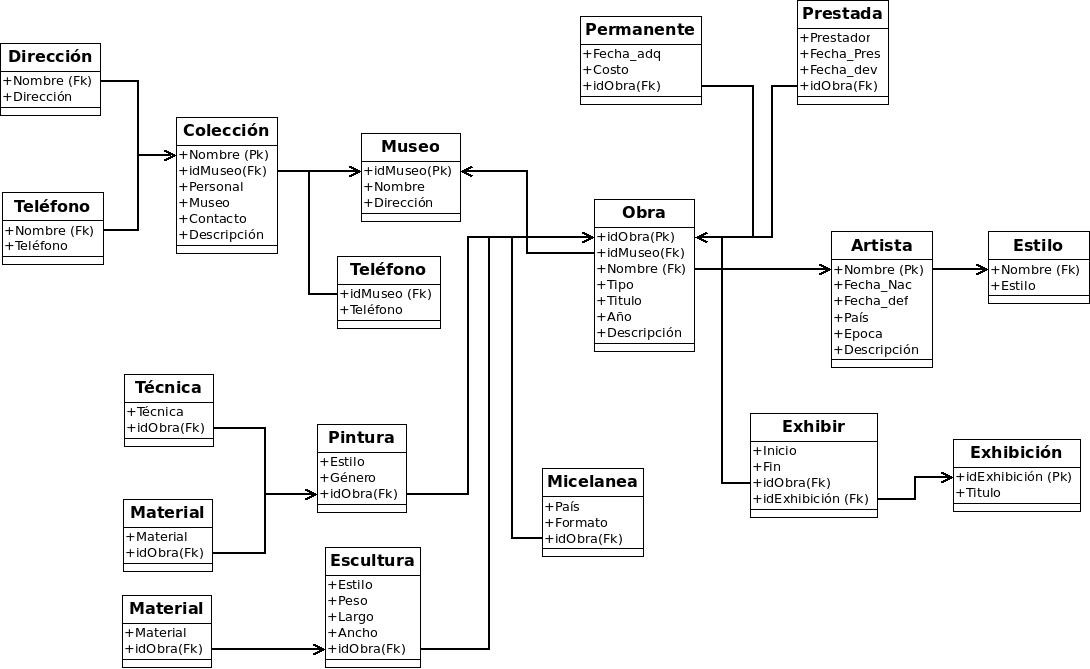
\includegraphics[scale=0.4]{img/museo.jpeg}
                \caption{Esquema relacional del Museo}
            \end{figure}
            \begin{enumerate}
                \item {
                    Toda la información de las obras, nombre del artista que la
                    realizó y país de las obras que se realizaron con estilo
                    Surrealista o Impresionista.
                    \begin{align*}
                        r &\leftarrow \sigma_{estilo = 'Surrealista'}(Estilo) 
                        \cup \sigma_{estilo = 'Impresionista'}(Estilo) \\
                        r &\leftarrow \pi_{nombre, pais}(Artista) \bowtie r \\
                        r &\leftarrow Obra \bowtie r
                    \end{align*}
                }
                \item {
                    Una lista con el nombre de los artistas y la cantidad de
                    obras que realizó (entre pinturas, esculturas y miscelánea).
                    \begin{align*}
                        r &\leftarrow \pi_{nombre}(Artista) \bowtie \pi_{nombre, 
                        idObra}(Obra) \\
                        r &\leftarrow (_{nombre}Y_{count(idObra)}(r)) \\
                        r &\leftarrow \rho_{numObras(count(idObra))}(r)
                    \end{align*}
                }
                \item {
                    Lista con la cantidad de obras que se tiene por cada estilo
                    (entre pinturas, esculturas y miscelánea).
                    \begin{align*}
                        r &\leftarrow Estilo \bowtie \pi_{nombre, idObra}(Obra) \\
                        r &\leftarrow (_{estilo}Y_{count(idObra)}(r)) \\
                        r &\leftarrow \rho_{numObras(count(idObra))}(r)
                    \end{align*}
                }
                \item {
                    Obtener el año en que menos obras se realizaron y la obra más
                    constosa de ese año.
                    \begin{align*}
                        r &\leftarrow (_{anio}Y_{count(idObra)}(Obra)) \\
                        r &\leftarrow \rho_{numObras(count(idObra))}(r) \\
                        minA &\leftarrow Min_{numObras}(r) \\
                        o &\leftarrow \sigma_{anio = minA}(\pi_{idObra, anio}(Obra)) \\
                        o &\leftarrow \pi_{costo, idObra}(Permanente) \bowtie o \\
                        maxP &\leftarrow (_{idObra}Y_{max_(precio)}(o)) \\
                        maxP &\leftarrow \pi_{idObra}(maxP) \bowtie Obra
                    \end{align*}
                }
                \item {
                    Toda información (obras y artistas) de las obras que se
                    obtuvieron en préstamo el 28 de noviembre de año 2014 y que
                    no han sido devuletas.
                    \begin{align*}
                        r &\leftarrow \pi_{idObra}(\sigma_{fechaPres = '28/11/2014' \land
                        fechaDev=null}(Prestada))\\
                        r &\leftarrow (Obra \bowtie r)\bowtie Artista
                    \end{align*}
                }
            \end{enumerate}
            \item {
                Si tienes el siguiente esquema para una Base de Datos:
                \begin{itemize}[label={}]
                    \item \textbf{Empleado}(CURP, nombre, calle, ciudad)
                    \item \textbf{Trabaja}(CURP, idEmpresa, sueldo)
                    \item \textbf{Empresa}(idEmpresa, nombre, ciudad)
                    \item \textbf{Jefe}(CURPJ, CURPE)
                \end{itemize}
                Considera que el sueldo que reciben los empleados es mensual.
                Escribe una expresión en \textbf{Álgebra Relacional} para cada
                una de las siguientes consultas
                \begin{enumerate}
                    \item {
                        Lista con la \textbf{CURP} y \textbf{nombre} de cada
                        empleado que trabaja en \textbf{Flanders Ship Asociados
                        (FSA)}.
                        \begin{align*}
                            r &\leftarrow \pi_{idEmpresa}(\sigma_{nombre = 
                            'Flanders Ship Asociados(FSA)'}(Empresa)) \\
                            r &\leftarrow \pi_{CURP}(Trabaja \bowtie r) \\
                            r &\leftarrow \pi_{CURP, nombre}(Empleado \bowtie r)
                        \end{align*}
                    }
                    \item {
                        Averiguar el \textbf{nombre} y la \textbf{ciudad de
                        residencia} de todos los empleados que trabajan para el 
                        \textbf{Compumundo Hipermega Red (CHR)}.
                        \begin{align*}
                            r &\leftarrow \pi_{idEmpresa}(\sigma_{nombre = 
                            'Compumundo Hipermega Red (CHR)'}(Empresa)) \\
                            r &\leftarrow \pi_{CURP}(Trabaja \bowtie r) \\
                            r &\leftarrow \pi_{nombre, ciudad}(Empleado \bowtie r)
                        \end{align*}
                    }
                    \item {
                        El \textbf{nombre}, \textbf{la calle} y la \textbf{ciudad
                        de residencia} de todos los empleados que trabajan para
                        \textbf{FSA} y ganan entre \textbf{\$150,000} y
                        \textbf{\$190,000} anuales.
                        \begin{align*}
                            r &\leftarrow \pi_{idEmpresa}(\sigma_{nombre = 
                            'Compumundo Hipermega Red (CHR)'}(Empresa)) \\
                            r &\leftarrow \sigma_{sueldo\geq 150000\land sueldo\leq 190000}
                            (Trabaja \bowtie r) \\
                            r &\leftarrow \pi_{CURP}(r) \bowtie Empleado\\
                            r &\leftarrow \pi_{nombre, calle, ciudad}(r)
                        \end{align*}
                    }
                    \item {
                        Encontrar el \textbf{nombre} y \textbf{CURP} de los
                        empleados que vivan en la misma ciudad en que está
                        ubicada la compañia a la que prestan sus servicios.
                        \begin{align*}
                            r &\leftarrow \rho_{ciudEmpr(ciudad)}(\rho_{nomEmpr(nombre)}
                            (Empresa))\\
                            r &\leftarrow (Empleado\bowtie Trabaja) \bowtie r\\
                            r &\leftarrow \pi_{nombre, CURP}(\sigma_{ciudad=ciudadEmpr}(r))
                        \end{align*}
                    }
                    \item {
                        Lista con el  \textbf{nombre} de los empleados que viven
                        en la \textbf{misma calle} y la \textbf{ciudad} de su jefe
                        \begin{align*}
                            cj &\leftarrow \rho_{CURP(CURPJ)}(\pi_{CURPJ}(Jefe)) \\
                            cj &\leftarrow \rho_{CURPJ(CURP)}(Empleado \bowtie cj)\\
                            cj &\leftarrow \rho_{ciudJ(ciudad)}(\rho_{calleJ(calle)}(cj))\\
                            cj &\leftarrow \pi_{CURPJ,calleJ,ciudJ}(cj) \\
                            ce &\leftarrow \rho_{CURP(CURPE)}(Jefe) \\
                            ce &\leftarrow (Empleado \bowtie ce) \\
                            ce &\leftarrow \pi_{CURPJ,calle,nombre,ciudad}(ce) \\
                            r &\leftarrow  (ce \bowtie cj)\\
                            r &\leftarrow \sigma_{calle == calleJ\land ciudJ == ciudad}(ce)\\
                            r &\leftarrow \pi_{nombre}(r) \\
                        \end{align*}
                    }
                    \item {
                        Averiguar la \textbf{CURP} de los empleados que no
                        trabajan para \textbf{FSA} pero sí para \textbf{CHR}.
                        \begin{align*}
                            r &\leftarrow \pi_{idEmpresa}(\sigma_{nombre = 'FSA'}(Empresa)) \\
                            r &\leftarrow \pi_{CURP}(Trabaja \bowtie r) \\
                            p &\leftarrow \pi_{idEmpresa}(\sigma_{nombre = 'CHR'}(Empresa)) \\
                            p &\leftarrow \pi_{CURP}(Trabaja \bowtie p) \\
                            r &\leftarrow r - p
                        \end{align*}
                    }
                    \item {
                        Encontrar el \textbf{nombre}, \textbf{CURP} y
                        \textbf{ciudad de residencia} de todos los jefes
                        registrados en la base de datos.
                        \begin{align*}
                            r &\leftarrow \rho_{CURP(CURPJ)}(\pi_{CURPJ}(Jefe)) \\
                            r &\leftarrow \pi_{nombre, CURP, ciudad}(r \bowtie Empleado)
                        \end{align*}
                    }
                    \item {
                        Una lista con el \textbf{nombre} de todos los empleados
                        que trabajan para  \textbf{CHR} pero no para
                        \textbf{FSA}.
                        \begin{align*}
                            r &\leftarrow \pi_{idEmpresa}(\sigma_{nombre = 'CHR'}(Empresa)) \\
                            r &\leftarrow \pi_{CURP}(Trabaja \bowtie r) \\
                            p &\leftarrow \pi_{idEmpresa}(\sigma_{nombre = 'FSA'}(Empresa)) \\
                            p &\leftarrow \pi_{CURP}(Trabaja \bowtie p) \\
                            r &\leftarrow r - p \\
                            r &\leftarrow pi_{nombre}(r \bowtie Empleado)
                        \end{align*}
                    }
                    \item {
                        Lista con la \textbf{CURP} de los empleados que ganan
                        más que cualquier empleado \textbf{FSA}.
                        \begin{align*}
                            r &\leftarrow \pi_{idEmpresa}(\sigma_{nombre = 'FSA'}(Empresa)) \\
                            m &\leftarrow Max_{sueldo}(Trabaja \bowtie r) \\
                            e &\leftarrow \pi_{CURP}(\sigma_{sueldo>m}(Trabaja))
                        \end{align*}
                    }
                    \item {
                        Lista con el \textbf{nombre de las companías} que están
                        instaladas en una ciudad donde haya un
                        \textbf{Krusty Burger}.
                        \begin{align*}
                            r &\leftarrow \pi_{ciudad}(\sigma_{nombre = 'Krusty Burger'}(Empresa)) \\
                            r &\leftarrow (Empresa \bowtie r) \\
                            r &\leftarrow \pi_{nombre}(r) \\
                        \end{align*}
                    }
                    \item {
                        Borrar toda la información de la companía
                        \textbf{Mapple}.
                        \begin{align*}
                            e &\leftarrow (\sigma_{nombre = 'Mapple'}(Empresa)) \\
                            t &\leftarrow (e \bowtie Trabaja) \\
                            t &\leftarrow \pi_{CURP,idEmpresa,sueldo}(t)\\
                            em &\leftarrow (Empleado \bowtie t) \\
                            em &\leftarrow \pi_{CURP,nombre,calle,ciudad}(em)\\
                            jf &\leftarrow \rho_{CURPJ(CURP)}(Jefe) \\
                            jf &\leftarrow (jf \bowtie t) \\
                            jf &\leftarrow \rho_{CURP(CURPJ)}(jf) \\
                            jf &\leftarrow \pi_{CURPJ,CURPE}(jf)\\
                            Empleado &\leftarrow Empleado - em\\
                            Trabaja &\leftarrow Trabaja - t\\
                            Empresa &\leftarrow Empresa - e\\
                            Jefe &\leftarrow Jefe - jf\\
                        \end{align*}
                    }
                    \item {
                        Disminuir el sueldo de los empleados que trabajan en
                        \textbf{Mr. Plow} en un \textbf{8\%}.
                        \begin{align*}
                            r &\leftarrow \pi_{idEmpresa}(\sigma_{nombre = 'Mr. Plow'}(Empresa)) \\
                            r &\leftarrow Trabaja \bowtie r \\
                            o &\leftarrow Trabaja - r \\
                            r &\leftarrow \pi_{CURP, idEmpresa, sueldo*1.08}(r)\\
                            r &\leftarrow \rho_{sueldo(sueldo*1.08)}(r)\\
                            Trabaja &\leftarrow r \cup o
                        \end{align*}
                    }
                    \item {
                        Una lista con la \textbf{cantidad de empleados} que se
                        tienen por ciudad y por compañía.
                         \begin{align*}
                            r &\leftarrow (Empresa \bowtie Trabaja)\\
                            r &\leftarrow _{idEmpresa,ciudad}Y_{Count(CURP)}(r)\\
                            r &\leftarrow \rho_{numerodeEmpleados(Count(CURP))}(r)\\
                            r &\leftarrow \pi_{idEmpresa,ciudad,numeroEmpleados}(r)\\
                         \end{align*}
                    }
                    \item {
                        Cambiar la ubicación de \textbf{Sorby} (y de 
                        \textbf{todos sus empleados}) a \textbf{Ciudad Capital}.
                         \begin{align*}
                            r &\leftarrow (\sigma_{nombre = 'Sorby'}(Empresa))\\
                            cte &\leftarrow \pi_{idEmpresa}(r)\\
                            t &\leftarrow (Trabaja \bowtie cte)\\
                            t &\leftarrow \pi_{CURP}(t)
                            cte &\leftarrow (idEmpresa, ciudad='Ciudad Capital')\\
                            Empresa &\leftarrow Empresa - r \\
                            r &\leftarrow (\pi_{idEmpresa,nombre}(r) \bowtie cte)\\
                            Empresa &\leftarrow Empresa \cup r\\
                            cte &\leftarrow \pi_{CURP,ciudad}(cte \bowtie Trabaja)\\
                            em &\leftarrow \rho_{ciudadOld(ciudad)}(Empleado)\\
                            em &\leftarrow \pi_{CURP,nombre,calle}(em \bowtie t)\\
                            cte &\leftarrow (cte \bowtie em)\\
                            Empleado &\leftarrow Empleado - (t \bowtie Empleado)\\
                            Empleado &\leftarrow Empleado \cup cte\\
                         \end{align*}
                    }
                    \item {
                        A los empleados que trabajan en \textbf{Ziffcorp} y que
                        ganen \textbf{\$18,000 mensuales} hacerles un
                        \textbf{decremento del 8\%}, mientras que a los que
                        trabajan en \textbf{Panaphonics} y que ganen 
                        \textbf{menos de \$12,000 mensuales} aumentarles su
                        sueldo en un \textbf{10\%}.
                         \begin{align*}
                         r & \leftarrow \sigma_{nombre = 'Ziffcorp' \wedge sueldo = 18 000 }(Trabaja \bowtie Empresa)\\
                         t & \leftarrow \pi_{CURP,idEmpresa,sueldo}(r)\\
                         r & \leftarrow \pi_{CURP,idEmpresa,sueldo*0.92}(r)\\
                         r & \leftarrow \rho_{sueldo(sueldo*0.92)}(r)\\
                         s & \leftarrow \sigma_{nombre = 'Panaphonics' \wedge sueldo < 12 000 }(Trabaja \bowtie Empresa)\\
                         w & \leftarrow \pi_{CURP,idEmpresa,sueldo}(s)\\
                         s & \leftarrow \pi_{CURP,idEmpresa,sueldo*1.1}(s)\\
                         s & \leftarrow \rho_{sueldo(sueldo*1.1)}(s)\\
                         Trabaja & \leftarrow Trabaja - t -w \\
                         Trabaja & \leftarrow Trabaja \cup r \cup s \\
                         \end{align*}
                    }
                    \item {
                        Lista de los empleados que trabajen en \textbf{más de
                        dos compañías} y el \textbf{número de companías} en que 
                        laboran.
                         \begin{align*}
                         r & \leftarrow _{CURP}Y_{count(idEmpresa)}(Trabaja)\\
                         r & \leftarrow \rho_{numComp(count(idEmpresa))}(r)\\
                         r & \leftarrow \sigma_{numComp > 2}(r)\\
                         \end{align*}
                    }
                    \item {
                        Lista que muestre la \textbf{CURP del jefe} y el
                        \textbf{número de empleados} que están a su cargo,
                        agrupados por companía.
                         \begin{align*}                         
                         r & \leftarrow _{idEmpresa,CURPJ}Y_{Count(CURPE)}(Empresa\bowtie_{CURP = CURPJ} Jefe )\\
                         r & \leftarrow \rho_{numerodeEmpleados(Count(CURPE))}(r)
                         \end{align*}
                    }
                    \item {
                        Una lista de los empleados que ganene \textbf{más de 
                        \$140,000 mensuales} y que \textbf{no viven} en
                        \textbf{Springfield}.
                        \begin{align*}
                        	r & \leftarrow \pi_{CURP,Nombre} (\sigma_{sueldo >140000}(Empleado \bowtie Trabaja))\\
                        	s & \leftarrow \pi_{CURP,Nombre} (\sigma_{ciudad= 'Springfield'\wedge sueldo >140000 }(Empleado \bowtie Trabaja))\\
                        	r & \leftarrow r-s\\                        	
                        \end{align*}
                    }
                    \item {
                        La empresa que paga el mayor \textbf{sueldo promedio}.
                        \begin{align*}
                        	r & \leftarrow _{idEmpresa}Y_{AVG(sueldo)}(Empresa \bowtie Trabaja)\\
                        	r & \leftarrow \rho_{SueldoProm(AVG(sueldo))}(r)\\
                        	s & \leftarrow Max_{SueldoProm}(r)\\
                        	r & \leftarrow \sigma_{SueldoProm = s}(r)\\
                        \end{align*}
                    }
                    \item {
                        \textbf{Moe Szyslak} decide dejar su bar y entrar a
                        trabajar a la planta nuclear, siendo su nuevo jefe
                        \textbf{Carl Carlson}. Refleja estos cambios en la base
                        de datos.
                        \begin{enumerate}
                        	\item  Suponiendo que el bar de Moe no es una empresa
                        	\begin{align*}
                        	r & \leftarrow Empleado \cup \{(CURP = 'curpMoe', nombre = 'MoeSzyslak',calle = 'c1', ciudad = 'Springfield')\}\\
                        	idPN & \leftarrow \pi_{idEmpresa}(\sigma_{nombre='PlantaNuclear'}(Empresa))\\
                        	Trabaja & \leftarrow Trabaja \cup \{(CURP = 'curpMoe',idEmpresa = idPN, sueldo = x)\}\\
                        	cCarl & \leftarrow \pi_{CURP}(\sigma_{nombre = 'Carl Carlson'}(Empleado)) \\
                        	Jefe & \leftarrow Jefe \cup \{(CURPJ = cCarl, CURPE = 'curpMoe')\} \\
                        	\end{align*}
                        	\item Suponiendo que el bar de Moe si es una empresa
                        	\begin{align*}
                        	c & \leftarrow \pi_{CURP}(\sigma_{nombre = 'Moe Szyslak'}(Empleado) )\\
                        	cCarl & \leftarrow \pi_{CURP}(\sigma_{nombre = 'Carl Carlson'}(Empleado)) \\
                        	idPN & \leftarrow \pi_{idEmpresa}(\sigma_{nombre='PlantaNuclear'}(Empresa))\\
                        	t & \leftarrow \rho_{idE(idEmpresa)}(idPN)\\
                        	r & \leftarrow \sigma_{CURP = c}(Trabaja)\\
                        	s & \leftarrow \pi_{CURP,idE,sueldo}(r \bowtie t)\\
                        	s & \leftarrow \rho_{idEmpresa(idE)}(s)\\
                        	Trabaja & \leftarrow Trabaja - r\\
                        	Trabaja & \leftarrow Trabaja \cup s\\
                        	w & \leftarrow \sigma_{CURP = c} (Jefe)\\
                        	Jefe & \leftarrow Jefe - w\\
                        	Jefe & \leftarrow Jefe \cup \{(CURPJ = cCarl, CURPE = c)\} \\                           	
                        	\end{align*}
                        \end{enumerate}
                        
                    }
                \end{enumerate}
            }
        }
    \end{enumerate}
\end{document}
